\documentclass[../main.tex]{subfiles}
\begin{document}

\section*{Problem Set 4}
    Name: Fangyuan Lin, UC Berkeley, Class of 2024

\subsection*{3.9 Fact about Markov chain}
a) Prove that if $X\to Y\to Z$ forms a Markov chain, $X\perp Y|Z$ and $X\perp Z$ imply $X\perp Y$.
\begin{proof}
    My intuition tells me to use mutual information:\\
    We know that $I(X;Z|Y)=0$ by Markov property. If $X\perp Y|Z$ and $X\perp Z$, then $I(X;Y|Z)=0$ and $I(X,Z)=0$. I don't bother denoting the set corresponding to $X$ with $\hat{X}$ because after all, everything is a set in ZFC. I use $\mu^*$ and $\mu$ interchangeably.
    \begin{align*}
        I(X;Y) &= \mu^*(X\cap Y)\\
        &= \mu(X\cap Y - Z) + \mu(X\cap Y\cap Z)\\
        &= \mu(X\cap Y\cap Z) \hspace{5mm} \text{because $X\perp Y|Z$}\\
        &= \mu(X \cap Z ) - \mu(X\cap Z-Y) \hspace{5mm} \textbf{by additivity}\\
        &= 0 - 0 \hspace{5mm}\textbf{by assumption and Markov property respectively}\\
        &=0
    \end{align*}
\end{proof}
b) Prove that the implication in a)
 continues to be valid without the Markov property.
 \begin{proof}
     \begin{align*}
        I(X;Y) &= \mu^*(X\cap Y)\\
        &= \mu(X\cap Y - Z) + \mu(X\cap Y\cap Z)\\
        &= \mu(X\cap Y\cap Z) \hspace{5mm} \text{because $X\perp Y|Z$}\\
        &= \mu(X \cap Z ) - \mu(X\cap Z-Y) \hspace{5mm} \textbf{by additivity}\\
        &= 0 -  \mu(X\cap Z-Y)\hspace{5mm}\textbf{by assumption}\\
        &=0 \hspace{5mm} \text{by non-negativeity of shannon's information measure}
    \end{align*}
 \end{proof}

 \subsection*{3.10 Some conditional independence facts}
 a) Show that $Y\perp Z|T$ does not imply $Y\perp Z | (X,T))$
 \begin{proof}
     Here is a counterexample. We always this example: take $X,Y$ as independent coin tosses. $Z$ be their sum $\mod 2$. Let $T$ be something completely irrelevant (indepdent to all of them). Then $X, Y$ are indepdent given the useless information about $T$, but if we further know $X$, then $X,Y$ are deterministic of each other.
 \end{proof}
 
 b) Prove that $Y\perp Z|T$ implies $Y \perp Z |(X,T)$ conditioning on $X\to Y\to Z\to T$.
 \begin{proof}
     \begin{align*}
         I(Y;Z|X,T) &= \mu(Y\cap Z -X -T)\\
         &=\mu(Y \cap Z - T) - \mu(Y\cap Z\cap X-T) \hspace{5mm}\text{by additivity}\\
         &=0-\mu(Y\cap Z\cap X-T)\hspace{5mm}\text{by assumption}\\
         &=0 \hspace{5mm}\text{by non-negativity of shannon's information measure}
     \end{align*}
 \end{proof}
 \subsection*{3.11 Some more facts about Markov chains}
 a) Let $X\to Y\to (Z,T)$ form a Markov chain. Prove that $I(X;Z)+I(X;T)\leq I(X;Y)+I(Z;T)$.
 \begin{proof}

 We are given that $I(X;(Z,T)|Y)=0$\begin{align*}
     &=I(X;Z,T|Y)\\
     &= I(X;Z|Y)+I(X;T|Y,Z)\quad \text{by chain rule}.
 \end{align*} All the quantities above are $0$. Consider
     \begin{align*}
         I(X;Y)+I(Z;T)-I(X;Z)+I(X;T)\\
         &= I(X;T|Z,T)+I(Y;Z;T|X)+I(Z;T|X;Y)\\
         I(X;Y|Z,T)+I(Z;T)\\
         &\geq 0.
     \end{align*}
 \end{proof}
 b)Let $X\to Y\to Z\to T$ form a Markov chain. Determine which of the following inequalities always hold:
 \begin{itemize}
     \item $I(X;T) + I(Y;Z)\geq I(X;Z) + I(Y;T)$\begin{proof}
         Always true.\begin{align*}
             &I(X;T)+I(Y;Z)-I(X;Z)+I(Y;T)\\
             &=I(Y;Z|X,T)\\
             &\geq 0.
         \end{align*}
         \item $I(X;T)+I(Y;Z)-I(X;Y)+I(Z;T)$.\begin{proof}
             The information diagram doesn't guarantee this.
         \end{proof}
     \end{proof}
     \item $I(X; Y) + I(Z; T) \geq I(X; Z) + I(Y; T)$.\begin{proof}
         True, by looking at information diagram.
     \end{proof}
 \end{itemize}
 \subsection*{3.14 Some fact about independence}
 \textbf{Problem:} Prove that for random variables \(X, Y, Z,\) and \(T\),
\begin{align*}
&X \perp Z \mid Y \\
&(X, Y) \perp T \mid Z \\
&Y \perp Z \mid T \\
&Y \perp Z \mid X \\
&X \perp T
\end{align*}
\(\implies Y \perp Z\).
\begin{proof}
    
    
    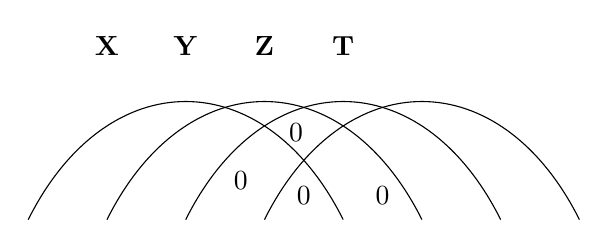
\begin{tikzpicture}
    % Draw the curves
    \draw (0,0) .. controls (1,2) and (3,2) .. (4,0);
    \draw (1,0) .. controls (2,2) and (4,2) .. (5,0);
    \draw (2,0) .. controls (3,2) and (5,2) .. (6,0);
    \draw (3,0) .. controls (4,2) and (6,2) .. (7,0);
    
    % Draw the labels
    \node at (1,2.2) {\textbf{X}};
    \node at (2,2.2) {\textbf{Y}};
    \node at (3,2.2) {\textbf{Z}};
    \node at (4,2.2) {\textbf{T}};
    
    % Draw the zeros
    \node at (3.5,0.3) {0};
    \node at (3.4,1.1) {0};
    \node at (2.7,0.5) {0};
    \node at (4.5, 0.3){0};
\end{tikzpicture}
\end{proof}
 \subsection*{3.15 Equivalence of 2 independence assumptions}
 Prove that
\[
X \perp Y, \quad X \perp Y \mid (Z, T), \quad Z \perp T \mid X, \quad Z \perp T \mid Y
\]
\(\iff\)
\[
Z \perp T, \quad Z \perp T \mid (X, Y), \quad X \perp Y \mid Z, \quad X \perp Y \mid T
\]
\begin{proof}
This is proven by drawing an information diagram and I find it tedious to include a latex diagram here.

\end{proof}
 \subsection*{4.5 Prove prefix code satisfies the Krafy inequality}
 \begin{proof}
     There are $D^{l_m}$ possible sequences of length $l_m$, some are codewords, some are children of codewords, and some are either. Note that for $l_i < l_m$, the number of children of length of order $l_m$ is $D^{l_m-l_i}$ and because the code is a prefix code, the sets of children of 2 different codewords are disjoint. \begin{align*}
         &\sum_{l_i<l_{m}}D^{l_m-l_i} + \sum_{l_i, l_i=l_m}1\quad\text{this is the number of all descendants of the codewords, with length $m$.}\\
         &=\sum_{i=1}^{m}D^{l_m-l_i}\\
         &\leq D^{l_m}\quad \text{because this is the total number of possible sequences of length $l_m$}
     \end{align*}
 \end{proof}
 \subsection*{4.7 Suffix code is uniquely decodable}
 \begin{proof}
     We can turn a suffix code into a prefix code by reversing the characters in the codewords.
 \end{proof}
 \subsection*{4.9 Random coding for prefix codes}
 Construct a binary prefix code with codeword lengths $l_1\leq \dots \leq l_m$ as follows. For each $1\leq k\leq m$, the codeword with length $l_K$ is chosen independenly from the set of all $2^{l_k}$ possible binary strings with length $l_k$ according the uniform distribution. Let $P_m(good)$ be the probability that the code so constructed is a prefix code.\\
 a) Prove that $P_2(good)=(1-2^{-l_1})^+$ where $(x)^+=\begin{cases}
     x \quad\text{if $x\geq 0$}\\
     =0 \quad \text{otherwise}
      \end{cases}$
\begin{proof}
  This part is straightforward. We only have $2$ codewords to worry about. \begin{align*}
      P_2(good) &= 1 - P_2(bad)\\
      &= 1 - P_2(\text{the second codeword is chosen to be a descendant of the first})\\
      &= 1 - 2^{l_1} \quad \text{the number of unavailable strings is $2^{l_2-l_1}$}
  \end{align*}
\end{proof}
 b) Prove by induction on $m$ that \begin{equation*}
     P_m(good) = \prod_{k=1}^m(1-\sum_{j=1}^{k-1}s^{-l_j})^+.
 \end{equation*}
 \begin{proof}
     Suppose \[
P_{n-1}(\text{good}) = \prod_{i=1}^{n-1} \left( 1 - \sum_{j=1}^{i-1} 2^{-l_j} \right).
\]. Then consider the number of available strings with length $l_n$ for the some prefix code $\C$.
 \end{proof}
 c) Observe that there exists a prefix code with codeword lengths $l_1,\dots,l_m$ if and only if $P_m(good) > 0$. Show that $P_m(good)>0$ is equivalent to the Kraft inequality.
 By using this random coding method, one can derive the Kraft inequality without knowing the inequality.
 \begin{proof}
     If there exists a prefix code, then there is a non-negative probability that we'll randomly generate it. If there exists no prefix code at all, $p_M(good)=0$.\\
     Suppose $P_m(good)>0$, then, then there exists a prefix $\C$ of the given lengths, then the lengths satisfy the Krafy inequality.\\
     If the lengths satisfy the Kraft inequality, $\sum s^{-l_i} \leq 1$, then we look at the formula in b). Note every term is positive in the product so $P_m(good)>0$
 \end{proof}
 \end{document}